\documentclass[10pt, journal]{IEEEtran}%,compsoc
\usepackage{ctex}
\usepackage{cite}
\usepackage{balance}  % to better equalize the last page
\usepackage{graphics} % for EPS, load graphicx instead
\usepackage{times}    % comment if you want LaTeX's default font
\usepackage{url}      % llt: nicely formatted URLs

\usepackage{graphicx}
\usepackage{subfigure}
\usepackage{subfigure}
\usepackage{helvet}
\usepackage{courier}
\usepackage{diagbox}
\usepackage{amsmath}
\usepackage{multirow}
\usepackage{booktabs}
\usepackage{makecell}
\usepackage{amssymb}
\usepackage{threeparttable}
\usepackage[justification=centering]{caption}
\usepackage[linesnumbered,ruled,vlined,commentsnumbered]{algorithm2e}
\usepackage{color}
\usepackage{xcolor}
%\usepackage{multirow}
%\usepackage[table]{xcolor}
\usepackage{colortbl}
\usepackage{float}
\usepackage{bm}
\usepackage[normalem]{ulem} % use normalem to protect \emph
\newcommand\hl{\bgroup\markoverwith
  {\textcolor{yellow}{\rule[-.5ex]{2pt}{2.5ex}}}\ULon}

\usepackage{Cite}

\ifCLASSINFOpdf

\else

\fi

\hyphenation{op-tical net-works semi-conduc-tor}

\usepackage{hyperref}
\usepackage{breakurl}
\newtheorem{definition}{Definition}
\def\boxend{\hspace*{\fill} $\Box$}
\newcommand{\comment}[1]{}
\renewcommand{\multirowsetup}{\centering}

\begin{document}

\title{Analyzing the Restoring Impact of Uplift Events on Overwhelmed Teenagers via Microblogs}

\author{Qi~Li,~Yuanyuan~Xue,~Liang~Zhao~and~Ling~Feng~\IEEEmembership{Senior~Member,~IEEE}
\IEEEcompsocitemizethanks{\IEEEcompsocthanksitem
\hspace{-0.3cm}
$^1$Faculty of Psychology,
Beijing Normal University, Beijing, China;\protect\\
$^2$Dept. of Computer Science and Technology,
Centre for Computational Mental Healthcare Research,
Tsinghua University, Beijing, China;\protect\\
$^3$Institute of Social Psychology, Xi'an Jiaotong University, Xi'an, China.\protect\\
E-mail: \{liqi2018\}@bnu.edu.cn,\{xue-yy12\}@mails.tsinghua.edu.cn,\{fengling\}@tsinghua.edu.cn,
\{zhaoliang0415\}@xjtu.edu.cn,
}}

\IEEEtitleabstractindextext{
\begin{abstract}
......
\end{abstract}

\begin{IEEEkeywords}
uplift event, adolescent, stress, microblogs
\end{IEEEkeywords}
}

\maketitle.

\IEEEdisplaynontitleabstractindextext

\IEEEpeerreviewmaketitle
\section{Introduction}
\paragraph{Stress} Life is always full of ups and downs.
The serious mental health problems caused by stress has become hot issues that are widely concerned around the world.
According to APA's newest report in 2018,
America��s youngest adults are most likely of all generations to report poor mental health,
and 91 percent of Gen Zs between ages 18 and 21 say they have experienced physical or emotional symptom due to stress in the past month compared to 74 percent of adults overall \citeauthor{APA2018}.
Accumulated stress comes from daily hassles, major stressful events and environmental stressors could drain people's inner resources,
leading to psychological maladjustment, ranging from depression to suicidal behaviours \citeauthor{Nock2008Suicide}.
Nowadays more than 30 million Chinese teenagers are suffering from psychological stress,
and nearly 30\% have a risk of depression \citeauthor{ChinaTeen2019}.
%1.����ѹ�����������

\paragraph{Restoring} As an important concept in psychological theory,
restoring is an essential process in human's stress coping system \citeauthor{Susan1984Stress}.
Timely and efficient restoring of stress could help teenagers get out of overwhelmed status.
%2.����ѹ���ͻ����ԭ��

����̽�󻺽�����ѹ���Ķ���;����
���У���ͳ����ѧ�о������������¼��ܹ���������ѹ����1��2��3����
���Ǿ���Ļ���ģʽ���д�̽����

�����罻ý�����������Ϊ̽���û���������״̬�ṩ�˼�ʱ/���������;����
ǰ���о�������ͨ���罻�������ݣ����Լ������ѹ����ѹ��Դ�¼���Ԥ��δ������ѹ�����Ƶȣ��ǿ��еģ��ɿ��ġ�
���ڻ����¼���̽����ؽ��չ�����Ӷ�Ϊ��ʱ��������ѹ����Ԥ��׼ȷԤ������ѹ����δ����չ�����ṩ��Ҫ��Ϣ��

�����罻�����о������¼���������ѹ���Ļ������ã���������һЩ���ѡ�
1��2��3��

���������ս�����ĵ���Ҫ���װ�����
1��2��3��


%Previous research has explored the possibility of detecting teenagers' stress series and
%mining the impact of stressor events from social media.
%On the contrary, the research on auto-analyzing the restoring ability of uplift events still calls for more exploration,
%due to the uncertainty and complexity of various restoring situations.
%In this paper,
%we give a deep inside into the stress easing function of uplift events on the real data set of 124 high school students.
%A two-sample based statistical model is conducted to analyze the stressful behavioral correlations
%when uplift events happened to overwhelmed students from multiple perspectives.
%Experimental results show that our method could measure the restoring impact of school scheduled uplift events with 69.52\% accuracy,
%and integrating such impact of uplift events helps reduce the stress prediction errors efficiently (with MSE, RMSE, MAPE and MAD reduced by 49.34\%, 28.81\%, 26.80\% and 42.11\%, respectively).
%Our exploration provides guidance for school and parents that which kind of uplift events could help relieve students' overwhelmed stress in both stress prevention and stress early stopping situations.


\section{Related Work}

\section{Method}

\section{Study1:}
\section{Study2:}
\section{Study3:}

\section{Discussion}

\section{Conclusion}
In this section, ...
\cite{Alden2008Social}


%\section{Introduction}
Life is always full of ups and downs.
According to the transactional model of stress \cite{Susan1984Stress}, our stress mainly comes from daily hassles.
The cumulative stress caused by the small and frequent stressful life events could drain people's inner resources,
leading to psychological maladjustment, ranging from depression to suicidal behaviours \cite{Nock2008Suicide}.
As a global public health concern,
suicide caused by psychological stress has become the second leading cause of death among young adults in college
(Centers for Disease Control and Prevention, 2012).

On the other hand, positive life events (called \emph{uplifts} in psychological theory) such as satisfying social interactions,
excellent academic performance and pleasant entertainment activities are conceptualized in psychological literature as exerting a protective effect on emotional distress \cite{Cohen1984Positive} \cite{Cohen2010Positive} \cite{Needles1990Positive}.
Compared with adults, young people exhibit more exposure to uplift events, as well as hassles,
due to the immature inner status and lack of experience \cite{older}.
Researchers indicate that positive events mitigate the relation between negative events and maladjustment in samples of adolescents experiencing family transitions \cite{Doyle2003Positive}.
The written expression of positive feelings has also be shown to prompt increased cognitive re-organization among an undergraduate student group \cite{Coolidge2009A}.

Positive uplifts can not only help reinforce adolescents' sense of well-being,
and help restore the capacity for dealing with stress,
but also have been linked to medical benefits, such as improving mood, serum cortisol levels, and lower levels of inflammation and hypercoagulability \cite{Jain2010Effects}.
Through examining the relationship between self-reported positive life events and blood pressure (BP) in 69 sixth graders,
researchers found that  increased perceptions of positive life events might act as a buffer to elevated BP in adolescents
\cite{Caputo1998Influence}.

The protective effect of uplift events is hypothesized to operate in two ways:
directly and indirectly by 'buffering' \cite{Cohen2010Positive}.
In the direct way,
the more positive uplift events people experienced, the less distress they experience.
While in the indirectly way, positive life events play its role by buffering the effects of negative events on distress.
A pioneer experiment conducted by Reich and Zautra provided enlightening evidence for us \cite{Shahar2002Positive}.
In this experiment, sampled college students who reported initial negative events were encouraged to engage in either two or twelve pleasant activities during one-month, and compared with students in the controlled group experiencing no pleasant activities.
Results indicated that participants in the two experimental groups reported greater quality of life compared with controlled students,
and participants who engaged in twelve uplift events exhibited lower stress compared with whom engaging two or none uplifts,
implicating the protective effect of uplift events on adolescents.

Previous exploration for the protective effect of uplift events on adolescents are mostly conducted in psychological area,
relying on traditional manpower-driven investigation and questionnaire.
The pioneer psychological researches provide us valuable implications and hypothesis,
while limited by labor cost, data scale and single questionnaire based method.
With the high development of social networks,
today adolescents tend to express themselves and communicate with outside world through posting microblogs,
at anytime and anywhere.
The self-motivated expressions could deliver much information about their inner thoughts and life styles.
In recent years, some research on psychological stress analysis based on social network has emerged,
from basically detecting stress intensity from microblog content
\cite{XueUbicomp13,Xue2014Detecting}, predicting future stress level in time series
\cite{Li2015Predicting,Li2015When,Li2015Using,Li2017Exploring},
to extracting stressor events and stressful intervals \cite{Li2017Analyzing}.
These researches explored applying psychological theories into social network based stress mining,
offering effective tools for adolescent stress sensing.
Nevertheless, few work takes an insight into the restoring function of uplift events,
which plays an important role opposite to stress,
as the essential way for adolescent psychological stress easing.

In this paper,
we aim to continually mine the restoring impact of uplift events leveraging abundant data source from microblogs,
to further provide guidance for school and parents that when and which kind of uplift events could help relieve students' overwhelmed stress in both stress prevention and stress early stopping situations.
To model such a practical application problem, several challenges exist.

\begin{itemize}
\item \emph{How to extract uplift events from microblogs and identify corresponding impact interval}?
The impact of uplift events is highlighted when the teen is under stress, with various relative temporal order.
Extracting such scenarios from teen's messy microblogs is the first and basic challenge for further analysis.
\item \emph{How to qualitatively and quantitatively measure the restoring impact conducted by uplift events}?
There are multiple clues related to teens' behaviours from microblogs, i.e.,
depressive linguistic content, abnormal posting behaviours.
The teen might act differently under similar stressful situations when the uplift event happens or not.
It is challenging to find such hidden correlation between uplift events and teen's behavioural characters.
\end{itemize}
Moreover, for different types of uplift events, the restoring impact might be different.
And for each individual, the protective and buffering effect for stress might also varies according to the personality.
All these questions guide us to solve the problem step by step.

In this paper, we first conduct a case study on real data set
to observe the posting behaviours and contents of stressful teens under the influence of uplift events.
We conduct the case study on the real data set of 124 high school students associated with the school's scheduled uplift and stressor event list.
Several observations are conducted to guide the next step research.
Next, we extract uplift events and the corresponding impacted interval from microblogs.
We define and extract structural uplift events from posts using linguistic parser model based
on six-dimensional uplift scale and LIWC lexicons.
Independent stressful intervals (SI) and stressful intervals impacted by uplifts (U-SI) are extracted considering temporal orders.
To quantify the restoring impact of uplift events,
we describe a teen's stressful behaviours in three groups of measures (stress intensity, posting behaviour, linguistic),
%to uniform
and model the impact of uplift events as the statistical difference between the sets of SI and U-SI in two aspects:
the two-sample based method is employed for variation detection,
and the t-test correlation is conducted to judge the monotonous correlation.

%to be add. 升华一下:意义是什么?

The rest of the paper is organized as follows.
We introduce related works in section \ref{sec:related}, 
and conduct the data observation in section \ref{sec:obs}.
The preliminaries and problem formulation are presented in section \ref{sec:problem}.
We conduct the procedure for extracting uplift events and identifying the impact interval in section \ref{sec:interval},
and introduce the detailed method for analyzing the restoring impact of uplift events in section 
\ref{sec:impact}. 
We present the experimental results in section \ref{sec:experiment}, 
and discuss the future work in section \ref{sec:conclude}.
%\section{Related Work}
\label{sec:related}
\subsection{Protective function of uplift events}
Many psychological researchers have focused on the restorative function of positive events and emotions with respect to physiological, psychological, and social coping resources.
Folkman \emph{et al.}\cite{Folkman2010Stress} identified three classes of coping mechanisms that are associated with positive emotion during chronic stress: positive reappraisal, problem-focused coping, and the creation of positive events.
The author also considered the possible roles of positive emotions in the stress process, and incorporated positive emotion into a revision of stress and coping theory in the work \cite{Folkman1997Positive}.
They conducted a longitudinal study of the care giving partners of men with AIDS and described coping processes that were associated with positive psychological states in the context of intense distress.
Cohen \emph{et al.} \cite{Cohen2010Positive} hypothesized that protective effect of uplift events operates in both directly (i.e., more positive uplift events people experienced, the less distress they experience) and indirectly ways by 'buffering'.

Chang \emph{et al.} \cite{Chang2015Loneliness} investigated the protective effect of positive events in a sample of 327 adults, and found that the positive association between loneliness and psychological maladjustment was found to be weaker for those who experienced a high number of positive life events, as opposed to those who experienced a low number of positive life events.
This is assistant with the conclusion made by Kleiman \emph{et al.}
\cite{Evan2014Social} that positive events act as protective factors against suicide individually and synergistically when they co-occur, by buffering the link between important individual differences risk variables and maladjustment.
Through exploring naturally occurring daily stressors, Ong \emph{et al.}
\cite{Ong2006Psychological} found that over time,
the experience of positive emotions functions to assist high-resilient individuals to recover effectively from daily stress.
In the survey made by Santos \emph{et al.} \cite{Santos2013The}, strategies of positive psychology are checked as potentially tools for the prophylaxis and treatment of depression, helping to reduce symptoms and for prevention of relapses.
Through a three-week longitudinal study, Bono \emph{et al.}
\cite{Bono2013Building} examined the correlation between employee stress and health and positive life events, and concluded that naturally occurring positive events are correlated with decreased stress and improved health.

\subsection{Measuring the Impact of Uplift Events}
To measure the impact of uplift events,
Doyle \emph{et al.} \cite{Kanner1981Comparison} conducted \emph{Hassles and Uplifts Scales},
and concluded that the assessment of daily hassles and uplifts might be a better approach to the prediction of adaptational outcomes than the usual life events approach.
Silva \emph{et al.} \cite{Silva2008The} presented the \emph{Hassles \& Uplifts Scale} to assess the reaction to minor every-day events in order to detect subtle mood swings and predict psychological symptoms.
To measure negative interpretations of positive social events,
Alden \emph{et al.} \cite{Alden2008Social} proposed the interpretation of positive events scale (\emph{IPES}), and analyzed the relationship between social interaction anxiety and the tendency to interpret positive social events in a threat-maintaining manner.
Mcmillen \emph{et al.} \cite{Mcmillen1998The} proposed the \emph{Perceived Benefit Scales} as the new measures of self-reported positive life changes after traumatic stressors, including lifestyle changes, material gain, increases in selfefficacy, family closeness, community closeness, faith in people, compassion, and spirituality.
Specific for college students,
Jun-Sheng \emph{et al.} \cite{Jun2008Influence} investigated in 282 college students using the \emph{Adolescent Self-Rating Life Events Checklist}, and found that the training of positive coping style is of great benefit to improve the mental health of students.

\subsection{Analyzing adolescent stress from social media}
With the high development of social network,
researchers tend to digging user' psychological status from the self-expressed public data source.
Billions of people record their life, share multi-media content, and communicate with friends through such platforms, e.g.,
Tencent Microblog, Twitter, Facebook and so on.
Inspired by rich microblogging content,
Xue \emph{et al.} \cite{XueUbicomp13, Xue2014Detecting} proposed to detect adolescent stress from single microblog utilizing machine learning methods by extracting stressful topic words, abnormal posting time, and interactions with friends.
Lin \emph{et al.} \cite{Lin2014User} construct a deep neural network to combine the high-dimensional picture semantic information into stress detecting.
Based on the stress detecting result,
Li \emph{et al.} \cite{Li2015Predicting}\cite{Li2015Using}\cite{Li2015When} adopted a series of multi-variant time series prediction techniques (i.e., Candlestick Charts, fuzzy Candlestick line and  SVARIMA model) to predict the future stress trend and wave.
Taking the linguistic information into consideration,
Li \emph{et al.} \cite{Li2017Exploring} employed a NARX neural network to predict a teen's future stress level referred to the impact of co-experiencing stressor events of similar companions.
All above pioneer work focused on the generation and development of teens' stress, providing solid basic techniques for broader stress-motivated research from social networks.

To find the source of teens' stress, previous work \cite{Li2017Analyzing} developed a frame work to extract stressor events from microblogging content and filter out stressful intervals based on teens' stressful posting rate.
Based on such research background, this paper starts from a completely new perspective, and focuses on the buffering effect of positive events on restoring stress.
Thus we push forward the study from how to find stress to the next more meaningful stage: how to deal with stress.

\subsection{Correlation analysis for multivariate time series}
Basic correlation analysis methods on time series focused on univariate data have been well studied.
As the most widely adopted method,
the Pearson correlation analysis \cite{Cohen1988Statistical} measures the linear correlation between two variables $X$ and $Y$.
One inevitable defect is that Pearson correlation is too sensitive to outlier values.
To overcome such drawback,
Spearman Rank correlation \cite{C1987The}
and Kendall Rank correlation \cite{Mcleod2011Kendall}
are proposed based on Pearson correlation.
While Pearson correlation estimates linear relationships,
Spearman correlation estimates monotonic relationships (whether linear or not),
and are calculated as the Pearson correlation between the rank values of two variables.
The Kendall correlation mainly assesses the similarity of the orderings of the data when ranked by each of the quantities.
The above correlation methods are usually used to estimate relationship between single-dimensional variables,
and cannot be adopted directly in our microblog content based scenario.

For multivariate time series analysis, two-sample based methods are widely adopted.
Such kind of methods are deduced to check whether two samples come from the same underlying distribution, which is assumed to be statistically unknown.
Correspondingly, various kernel
\cite{Sch2006A} and distance-based methods \cite{Schilling1986Multivariate}
(e.g., the nearest neighbor based method two-sample method) are proposed.
Scholkopf \emph{et al.} \cite{Sch2006A} proposed to transform the distance between two variables and nearest neighbors into a reproducing kernel Hilbert space (RKHS), and solve the problem using Maximum Mean Discrepancy.
In work \cite{Schilling1986Multivariate},
Schilling \emph{et al.} adopted the $r$-nearest neighbor based method to partition two set of event driven time series data.
The global proportion of the right divided neighbors are calculated to estimate whether there exists statistically difference between the two sets.
We use the $r$-nearest neighbor based two-sample method in our problem, thus to measure the distance and correlation between two multi-dimension variables.

%\begin{table}
\begin{center}
\caption{Examples of uplift events expressed and extracted from teens' microblogs.}
\begin{tabular}{l} \hline \rowcolor{gray!40}
I am really looking forward to the spring outing on Sunday now. \\ \rowcolor{gray!40}
(Doer:\emph{I}, Act:\emph{looking forward}, Object:\emph{spring outing})\\
My holiday is finally coming [smile]. \\
(Doer:\emph{My holiday}, Act:\emph{coming}, Object:\emph{[smile]})\\ \rowcolor{gray!40}%\hline
First place in my lovely math exam!!! In memory of it.\\ \rowcolor{gray!40}
Object:\emph{first place, math, exam, memory})\\ %\hline
You are always here for me like sunshine. \\
(Doer:\emph{You}, Object:\emph{sunshine})\\ \rowcolor{gray!40} %\hline
Thanks all my dear friends to take the party for me. Happiest birthday!\\ \rowcolor{gray!40}
(Doer:\emph{friends}, Act:\emph{thanks}, Object:\emph{party, birthday})\\
Be yourself. Trust yourself and follow your heart. \\
(Doer:\emph{yourself}, Act:\emph{trust}, Object:\emph{heart})\\ \rowcolor{gray!40} %\hline
Feel proud of our play in the Games. Our class is always the family!!!\\ \rowcolor{gray!40}
(Doer:\emph{Our}, Object:\emph{class, family})\\
A good film always makes bring comfort and happiness to me.\\
(Doer:\emph{me}, Act:\emph{bring}, Object:\emph{comfort, happiness})\\ \rowcolor{gray!40}%\hline
I know my mom is the one who support me forever, no matter \\ \rowcolor{gray!40}
when and where. (Doer:\emph{mom}, Act:\emph{support})\\ \hline
\end{tabular}
\label{tab:uplifts}
\end{center}
\end{table}

\begin{table}
\begin{center}
\caption{Examples of stressor events expressed and extracted from teens' microblogs.}
\begin{tabular}{l} \hline \rowcolor{gray!40}
I don't know how long can I bear the nag.\\ \rowcolor{gray!40}
(Doer:\emph{I}, Act:\emph{bear}, Object:\emph{nag})\\ %\hline
Parents like to judge everything around me with their emotion.
\\(Doer:\emph{parents}, Act:\emph{judge}, Object:\emph{everything})\\ \rowcolor{gray!40}%\hline
Hope that my uncle could revive earlier.\\ \rowcolor{gray!40}
(Doer:\emph{my uncle}, Act:\emph{revive})\\%\hline
Every one betrayed me.
\\(Doer:\emph{every one}, Act:\emph{betray}, Object:\emph{me})\\ \rowcolor{gray!40} %\hline
I'm too weak to handle such a fierce competition.\\ \rowcolor{gray!40}
(Doer:\emph{I}, Act:\emph{too weak to handle}, Object:\emph{competition})\\%\hline
I just felt hurt, depressed, self-abased and sad.
\\(Doer:\emph{I}, Act:\emph{feel hurt, depressed, self-abased and sad})\\ \rowcolor{gray!40}%\hline
My holiday is filled with all kinds of homework.\\ \rowcolor{gray!40}
(Doer:\emph{My holiday}, Act:\emph{fill with}, Object:\emph{homework})\\ %\hline
Unescapably, it's time to go back to school.
\\(Act:\emph{go back}, Object:\emph{school})\\ \rowcolor{gray!40} %\hline
When can you be aware of my heart-broken feeling again and again?\\ \rowcolor{gray!40}
(Doer:\emph{you}, Act:\emph{be aware of}, Object:\emph{heart-broken feeling})\\ \hline
\end{tabular}
\label{tab:stressors}
\end{center}
\end{table}

\begin{table}
\centering
\caption{Examples of school scheduled uplift events and stressor events.}
\label{tab:example}
\begin{tabular}{cccc}
\toprule
Type & Date	& Work Content	& Grade	\\
\midrule
\emph{stressor event} & 2014/4/16 & \emph{first day of mid-term exam} & grade1,2\\
\emph{uplift event} & 2014/11/5 & \emph{campus art festival} & grade1,2,3\\
\bottomrule
\end{tabular}
\end{table}

\begin{figure}
\centering
\caption{Examples of school related stressor events, uplift events and a student's stress fluctuation}
\includegraphics[width=\linewidth]{figs/exampleWave.eps}
\label{fig:example}
\end{figure}

\section{Data Observation}
\label{sec:obs}
We built our dataset based on two sources: 1) the microblogs of students coming from Taicang High School,
collected from January 1st, 2012 to February 1st, 2015;
and 2) list of scheduled school events, with exact start and end time.
We filtered out 124 active students according to their posting frequency from over 500 students,
and collected their microblogs throughout the whole high school career. Totally 29,232 microblogs are collected in this research,
where 236 microblogs per student on average, 1,387 microblogs maximally and 104 posts minimally.

\emph{Uplift events and stressor events}.
The list of weekly scheduled school events (from February 1st, 2012 to August 1st 2017) are collected from the school's official website
\footnote{http://stg.tcedu.com.cn/col/col82722/index.html}, with detailed event description and grade involved in the event.
There are 122 stressor events and 75 uplift events in total.
Here we give the examples of scheduled uplift and stressor events in high school life, as shown in Table~\ref{tab:example}.
There are 2-3 stressor events and 1-2 uplift event scheduled per month.


\emph{Stress detected from microblogs}.
Since our target is to observe the restoring impact of uplift events for teenagers under stress.
Based on previous research~\cite{XueUbicomp13},
we detected the stress level (ranging from 0 to 5) for each post;
and for each student, we aggregated the stress during each day by calculating the average stress of all posts.
The positive level (0-5) of each post is identified based on the frequency of positive words (see Section 5 for details).
Figure~\ref{fig:example} shows three examples of a student's stress fluctuation during three mid-term exams,
where the uplift event \emph{campus art festival} was scheduled ahead of the first exam,
the uplift event \emph{holiday} happened after the second exam,
and no scheduled uplift event was found nearby the third exam.
The current student exhibited differently in above three situations, with the stress lasting for different length and with different intensity.

To further observe the influence of uplift events for students facing stressor events,
we statistic all the stressful intervals~\cite{Li2017Analyzing} detected surround the scheduled examinations over the 124 students during their high school career.
For each student, we divide all his/her stressful intervals into two sets:
1) stressful intervals under the influence of neighbouring uplift events (e.g., \emph{Halloween activity}), and 2) independent stressful intervals.
Figure~\ref{fig:frequency} shows five measures of each student during the above two conditions:
the \emph{accumulated stress}, the \emph{average stress} (per day), the \emph{length of stressful intervals},
the \emph{frequency of academic topic words}, and the \emph{ratio of academic stress among all types of stress}.
For each measure, we calculate the average value over all eligible slides for each student.

\emph{Findings}. Comparing each measure in scheduled exam slides under the two situations: 1) existing neighbouring uplift events or 2) no neighbouring scheduled uplift events,
we find that students during exams with neighbouring uplift events exhibit less average stress intensity (both on accumulated stress and average stress),
and the length of stress slides are relatively shorter.
Further, we statistic the frequency of academic related topic words for each exam slide (as listed in Table \ref{tab:studyWords}),
and look into the ratio of academic stress among all five types of stress.
Results in Figure~\ref{fig:frequency} shows that most students talked less about the upcoming or just-finished exams when uplift events happened nearby,
with lower frequency and lower ratio.
The stress intensity and type distribution detected from each student's microblogs varies due to personal life experience, posting habits and express styles.
The statistic result shows clues about the stress-relieving ability of scheduled uplift events,
and thus helps shape our problem as how to quantify the influence of uplift events,
thus to provide further guidance for planning campus activities to help relive high school students' psychological stress effectively.

\begin{table}[h]
\centering
\caption{Examples of academic related topic words.}
\label{tab:studyWords}
\begin{tabular}{c}
\toprule
exam, fail, review, score, grade, test paper, rank, pass, math, chemistry\\
homework, recite, regress, fall behind, tension, stressed out, physics,\\
nervous, mistake, answer, question, puzzle, difficult, lesson, careless, \\
\bottomrule
\end{tabular}
\end{table}


\begin{figure}
\centering
\caption{Compare students' stress during exam intervals in two situations:
1) affected by neighboring uplift events (U-SI), 2) no uplift events occurred nearby (SI)}
\includegraphics[width=\linewidth]{figs/frequency.eps}
\label{fig:frequency}
\end{figure}


%\section{Preliminaries}
\label{sec:problem}
Based on the observation and psychological theory,
we conduct our research under the assumption that uplift events can ease teenagers' stress,
namely the positive restoring impact of uplift events.
While stressor events stimulate human's stress,
uplift events bring positive influence and stronger restoring ability to stressed people in various situations with multi-types~\cite{Cohen1984Positive}\cite{Cohen2010Positive}\cite{Needles1990Positive}.
Taking the three stress curves in Figure~\ref{fig:example} for example,
comparing the stress curves \emph{a)}, \emph{b)} with \emph{c)},
when an uplift event (\emph{campus art festival, holiday} here) happens,
the overall stress intensity during the stressful period is reduced.
An uplift event might happen before a teen's stress caused by scheduled stressor events (\emph{example a}),
conducting lasting easing impact;
Meanwhile, an uplift event might also happen during (\emph{example b}) or at the end of the stressful period,
which might promote the teen out of current stressful status more quickly.
To study the restoring impact of an uplift event, we structure its impact from three aspects:
\begin{itemize}
\item \textbf{Impact interval of uplifts}.
To study the impact of uplift events from microblogs,
two fundamental factors are identifying the exact time when the uplift event happens,
and the corresponding stressful interval it impacts.
The temporal order between uplift events and the teen's stress series varies in different situations,
and its a challenge to match the uplift event to the right stressful interval it actually impacts.
\item \textbf{Restoring patterns of uplifts}.
As the restoring impact of uplift events relieves the teen's stress and exhibits in multiple aspects
(e.g., the changes in posting behavior, linguistic expression, and stress intensity from microblogs),
it's meaningful to extract the stress-related restoring patterns and describe the restoring impact of uplift events structurally.
\item \textbf{Quantified impact of uplifts}.
Different types of uplift events might conduct restoring impact with different intensity.
In this paper, the ultimate problem we target to solve
is how to quantify the restoring impact both qualitatively and quantitatively from teenagers microblogs.
\end{itemize}

Given an uplift event with specific type,
we consider its restoring impact by comparing the teen's behavioral measures under two situations.
As illustrated in Figure \ref{fig:SI},
in the original situation (i.e., sub-series A),
the teen's stress is caused by a stressor event, lasting for a period,
and no other intervention (namely, uplift event) occurs.
We call the set of such stressful intervals as \textbf{SI}.
In the other comparative situation (i.e., sub-series B),
the teen's stressful interval caused by the same type of stressor is impacted by an uplift event with type $x$,
we call the set of such stressful intervals as \textbf{U-SI}.
Thus the difference under the two situations SI and U-SI could be seen as the restoring impact conducted by the uplift event of type $x$.

Next, we give the formal definition for uplift events and stressor events from the perspective of linguistic structure.

\begin{figure}
\centering
\caption{Illustration of SI and U-SI stressful intervals.}
\includegraphics[width=\linewidth]{figs/UpSeries.eps}
\label{fig:SI}
\end{figure}
\begin{definition}
\textbf{Uplift event}.
Let $u$ = $[type,\{role, act,$ $descriptions\}]$ be an uplift event,
where the element \emph{role} is the subject who performs the \emph{act},
and \emph{descriptions} are the key words related to $u$.
According to psychological scales \cite{hassles,Jun2008Influence},
teenagers' uplift stressors mainly focus on six aspects,
as $\mathbb{U} =\{$ \emph{entertainment', 'school life', 'family life',
'pear relation', 'self-cognition', 'romantic'}$\}$, $\forall u$, $u._{type} \in \mathbb{U}$.
\end{definition}

\begin{definition}
\textbf{Stressor event}.
Similar to stressor event,
let $e$ = $[type,\{role, act,$ $descriptions\}]$ be a stressor event.
According to psychological questionnaires \cite{Kanner1981Comparison, scale1, scale2, scale3},
we classify stressor events into five types, as $\mathbb{S}=\{$ \emph{'school life', 'family life',
'pear relation', 'self-cognition', 'romantic'}$\}$, $\forall e$, $e._{type} \in \mathbb{S}$.
\end{definition}

The examples of teens' microblogs describing uplift events and stressor events are listed in Table \ref{tab:uplifts} and Table \ref{tab:stressors}.
For the post '\emph{I have so much homework today!!!}', its elements are \emph{role = 'I', act='have', descriptions = 'homework'}, and the \emph{type = 'school life'}.
For the post '\emph{Expecting Tomorrow' Adult Ceremony[Smile][Smile]~~}', we translate it into \emph{act = 'expecting', description = 'Adult Ceremony'}, and the \emph{type = 'self-cognition'}.

\textbf{Problem}: For an uplift event $u$ with type $U^{'}$,
a stressor event $e$ with type $S^{'}$,
let $F$:$(u, U^{'}, e, S^{'}) \rightarrow $ \bm{${A}$}
(\bm{${A}$} is a multidimensional vector) be the restoring influence of uplift event $u$
conducted on the stress caused by stressor event $e$.
We aim to quantify such influence \bm{${A}$} from multiple views.

%\section{Identify Uplifts and Impact Interval}
\label{sec:interval}
In this section,
we first introduce the procedure to extract uplift events and stressful intervals from teens' microblogs.
The uplift events are extracted from microblogs applying LTP natural language processing segmentation and parser models
\cite{che2008}.
Stressful intervals are identified using probability based statistical method according to the teen's stressful posting frequency.
We judge whether each stressful interval is correlated with neighboring uplift events,
thus to classify all stressful intervals into two sets: SI and U-SI.

\subsection{Uplift Events}
\emph{Lexicon}.
We construct our lexicon for six-dimensional uplift events from two sources.
The basic positive affect words are selected from the psychological lexicon SC-LIWC (e.g., \emph{expectation}, \emph{joy}, \emph{love} and \emph{surprise})\cite{Tausczik2010The}.
Then we build six uplift event related lexicons by expanding the basic positive words from the data set of teens' microblogs,
and divide all candidate words into six dimensions corresponding to six types of uplift events,
containing 452 phrases in \emph{entertainment},
184 phrases in \emph{family life},
91 phrases in \emph{friends},
138 phrases in \emph{romantic},
299 phrases in \emph{self-recognition} and 273 phrases in \emph{school life}, with totally 2,606 words,
as shown in Table \ref{tab:keyWords}.
Additionally, we label \emph{role} words (i.e., \emph{teacher}, \emph{mother}, \emph{I, we}) in the uplift lexicon.

\emph{Parser relationship}.
For each post, after word segmentation, we parser current sentence to find its linguistic structure,
and then match the main linguistic components with uplift event related lexicons in each dimension.
The parser model in Chinese natural language processing platform \cite{Che2010, che2008} is adopted in this part,
which identifies the central verb of current sentence first, namely the \emph{act},
and constructs the relationship between the central verb and corresponding \emph{role} and \emph{objects} components.
By searching these main elements in uplift event related lexicons,
we identify the existence and type of any uplift event.
Due to the sparsity of posts, the \emph{act} might be empty.
The \emph{descriptions} are collected by searching all nouns, adjectives and adverbs in current post.
In such way, we extract structured uplift events from teens' microblogs.

\begin{table}
\centering
\caption{Examples of topic words for uplift events.}
\label{tab:keyWords}
\begin{tabular}{lll}
\toprule
Dimension & Example words & Total \\ \midrule
\emph{entertainment}  & hike, travel, celebrate, dance, swimming, ticket, & 452\\
& shopping, air ticket, theatre, party, Karaoke, & \\
& self-driving tour, game, idol, concert, movie, & \\
\emph{school life}       & reward, come on, progress, scholarship, & 273\\
				  & admission, winner, diligent, first place, superior, & \\
				  & hardworking, full mark,  praise, goal, courage, & \\
\emph{romantic}         &  beloved, favor, guard, anniversary,  concern,  & 138\\
				  & tender, deep feeling, care, true love, promise, & \\
				  & cherish, baby, kiss, embrace, dating, reluctant,&\\
\emph{pear relation}   & listener, company, pour out, make friends with, & 91\\
				 & friendship, intimate, partner, team-mate,&\\
\emph{self-cognition} & realize, achieve, applause, fight, exceed, faith, & 299\\
				 & confidence, belief, positive, active, purposeful, &\\
\emph{family life}       & harmony, filial, reunite, expecting, responsible, & 184\\
				& longevity, affable, amiability, family, duty, &\\
\bottomrule
\end{tabular}
\end{table}

\subsection{Impact Interval}
When an uplift event happens, it can conduct positive impact on stressed teens,
which may exhibit in multi-perspectives,
including the length of corresponding stressful interval, the stress intensity and stressful behaviors during the interval.
Basically, in this part, we identify stressful intervals from timeline thus to support further quantifying the influence of an uplift event.
Splitting interval is a common time series problem, and various solutions could be referred.
Here we identify the teen's stressful intervals in three steps.
In the first step, we extract uplift events, stressor events and filter out candidate intervals after a smoothing process.
Then, applying the Poisson based statistical method proposed in~\cite{Li2017Analyzing},
we judge whether each candidate interval is a confidential stressful interval.
Finally, we divide the stressful intervals into two sets: the SI set and the U-SI set,
according to its temporal order with neighboring uplift events.

\emph{Smooth stress series}.
Since a teen's stress series $S=\{s_1, s_2, \cdots, s_n\}$ detected from microblogs (aggrated by day) are discrete points,
we adopt the loess (local regression using weighted linear least squares and a $2^{nd}$ degree polynomial) method \cite{Cleveland1988Locally} to highlight characteristics of the stress curve.
In loess method, we need to set the parameter \emph{span},
which represents the percentage of the selected data points in the whole data set (ranging from 0 to 1),
and determines the degree of smoothing.
We discuss the influence of different \emph{span} settings on the result of interval segmentation in the experiment section.
%to be add 1: interval parameter.

\emph{Select candidate intervals.}
We filter out candidate stressful intervals on the smoothed stress series $S^{'}=\{s^{'}_1,s^{'}_2,\cdots,s^{'}_n\}$.
%As illustrated in Figure xx, w
Let the sub-series $w_{<a,b>} = [s^{'}_a, \cdots, s^{'}_b]$ as a \emph{wave},
where $s^{'}_v$ $= {vally(w_{<a,b>})}$ is the minimum stress value,
$s^{'}_p$ $= peak(w_{<a,b>})$ is the maximal stress value during $\{s^{'}_a,\cdots,s^{'}_b\}$,
and $s^{'}_a \leq s^{'}_{a+1} \leq \cdots \leq s^{'}_p \leq s^{'}_{p+1} \leq \cdots \leq s^{'}_b$.
A candidate interval $I = <w_1,\cdots, w_i,\cdots, w_m>$ is identified with following rules:
\begin{itemize}
\item $s^{'}_1 = 0$, $s^{'}_m = 0$. $\forall s^{'}_j \in \{s^{'}_2,\cdots,s^{'}_{m-1}\}$, $s^{'}_j > 0$.
\item Let wave $w_i$ be the biggest wave in current candidate interval, with $peak(w_i) = \omega$,
$\forall $ wave $w_j \in I$, $peak(w_j)<=peak(w_i)$.
\item For waves $w_k$ before the interval biggest wave $w_i$ , i.e., $\forall w_k \in <w_1,\cdots,w_{i-1}>$,
$peak(w_{k+1})>=peak(w_k)$, $vally(w_{k+1}) >= peak(w_k)$.
\item For waves $w_k$ behind the interval biggest wave $w_i$, i.e.,  $w_k \in <w_{i}, \cdots, w_m>$,
$peak(w_{k+1})<=peak(w_k)$, $vally(w_{k+1}) <= peak(w_k)$.
\end{itemize}

\emph{Identify stressful intervals.}
For each candidate interval,
a Poisson based probability model~\cite{Li2017Analyzing} is adopted to measure how confidently the current interval is a stressful interval.
Here a teen's stressful posting rate under stress ($\lambda_1$) and normal conditions ($\lambda_0$) are modeled as two independent poisson process:
\begin{equation}
Pr[N=n|\lambda_i]=\frac{e^{-\lambda_i T}{(\lambda_i T)}^n}{n!}
\end{equation}
where $i\in\{0,1\}$, $n=0,1,\cdots,\infty$.
We expect that $\lambda_1 > \lambda_0$, and measure the probability as $P(\lambda_1>\lambda_0|N_1, T_1, N_0, T_0)$,
where $N_1, N_0$ are the number of stressful posts, and $T_1, T_0$ are time duration corresponding to $\lambda_1$ and $\lambda_0$.
Without loss of generality, we assume a Jeffreys non-informative prior on $\lambda_1$ and $\lambda_0$,
and infer the posterior distribution $P(\lambda_1|N_1)$ and $P(\lambda_0|N_0)$ according to Bayes Rule.
Thus for current interval $I_1$ and historical normal interval $I_0$,
the quantified probability $\beta = P(\lambda_1>\lambda_0|I_1,I_0)$ $\in (0,1)$ indicates the confidence whether $I_1$ is a stressful interval.

\emph{Intervals impacted by uplift events.}
In this part, we filter out two sets of stressful intervals: stressful intervals without the impact of uplift events (SI),
and stressful intervals under the impact of uplift events (U-SI).
For a detected stressful interval $I = <t_1,\cdots,t_n>$, we consider the temporal order between $I$ and any detected uplift event $u$ happened at time point $t_u$:
\begin{itemize}
\item If the uplift event $u$ happens during the stressful interval, i.e., $t_u \in [t_1,t_n]$, the uplift interval $I$ is judged as $I \in SI$.
\item For the uplift event happening nearby a stressful interval,
we also consider the probability that it conducts impact on the teen's stressful interval.
Here the gap between $t_u$ and $I$ is limited to $\xi$, i.e.,
if $t_u \in [t_{1}-\xi, t_1)\cup(t_{n},t_{n}+\xi]$, then $I \in SI$.
%The setting of parameter $\xi$ is discussed in experiment section.
\end{itemize}
If a stressful interval satisfies none of the above conditions, we classify it into the U-SI set.


%\section{Impact of Uplift Events}
\label{sec:impact}
To quantify the restoring impact of uplift event,
in this section, we propose to model the impact as the teen's behavioral differences in two cases:
1) stressful intervals unaffected by uplift events (SI), and 2) stressful intervals impacted by uplift events (U-SI).
Multiple stress and positive emotion related measures are proposed to describe the correlation between SI and U-SI,
and we quantify such differences as correlations using a two-sample based statistical method.

\subsection{Restoring Patterns and Behavioral Measures}
\label{subsec:pattern}
To extract the restoring patterns of each type of uplift events,
we describe a teen's positive and stressful behavioral measures in SI and U-SI sets from three aspects:
posting behavior, stress intensity, and linguistic expressions.

\textbf{Posting behavior}.
Stress could lead to a teen's abnormal posting behaviors,
reflecting the teen's changes in social engagement activity.
For each stressful interval,
we consider three measures of posting behaviors in each time unit (day),
and present each measure as a corresponding series.
The first measure is \emph{posting frequency},
representing the total number of posts per day.
Research in \cite{Li2017Analyzing} indicates that overwhelmed teens usually tend to post more to express their stress for releasing
and seeking comfort from friends.
Further, the second measure \emph{stressful posting frequency} per day
is based on previous stress detection result and highlights the stressful posts among all posts.
Similarly, the third measure is the \emph{positive posting frequency}, indicating the number of positive posts per day.
The forth measure \emph{original frequency} is the number of original posts, which filters out re-tweet and shared posts.
Compared to forwarded posts, original posts indicate higher probability that teens are talking about themselves.
Thus for each day in current interval, the teen's posting behavior is represented as a four-dimension vector.

\textbf{Stress intensity}.
We describe the global stress intensity during a stressful interval through four measures:
\emph{sequential stress level, length, RMS,} and \emph{peak}.
Basically, \emph{stress level} per day constructs a sequential measure during a stressful interval,
recording stress values and fluctuation on each time point.
The \emph{length} measures the lasting time of current stressful interval.
As uplift events might conduct impact on overwhelmed teens,
and postpone the beginning or promote the end of the stressful interval,
we take the \emph{length} as a factor representing the interval stress intensity.
To quantify the intensity of fluctuations for stress values,
we adopt the \emph{RMS} (root mean square) of stress values through the interval as the third measure.
In addition, the \emph{peak} stress value is also a measure to show the maximal stress value in current interval.

\textbf{Linguistic expressions}.
We extract the teen's positive and stressful expressions from the content of posts in SI and U-SI sets, respectively.
The first linguistic measure is the frequency of \emph{positive word},
which represents the positive emotion in current interval.
The second measure is the frequency of \emph{uplift event topic words} in six dimensions,
reflecting the existence of uplift events.
Another important factor is wether existing \emph{self-mentioned words} (i.e., \emph{'I','we','my'}).
Self-mentioned words show high probability that the current stressor event and stressful emotion is related to the author,
rather than the opinion about a public event or life events about others.

Except uplift-related linguistic descriptions, we also take stressful linguistic characters as measures,
which is opposite with positive measures, while also offers information from the complementary perspective.
The first stressful linguistic measure is the frequency of \emph{stressor event topic words} in five dimensions,
which represents how many times the teen mentioned a stressor event,
indicating the degree of attention for each type of stressor event.
The frequency of \emph{pressure words} is the second stressful linguistic measure,
reflecting the degree of general stress emotion during the interval.
We adopt this measure specifically because in some cases teens post very short tweets with only stressful emotional words,
where topic-related words are omitted.

Next,
based on the posting behavior, stress intensity and linguistic measures from both the stressful and positive views,
we quantify the difference between SI and U-SI sets, thus to measure the impact of uplift events.

\subsection{Quantify the Correlation}
In our problem,
there are two sets of stressful intervals to compare:
the SI set and the U-SI set,
containing stressful intervals unaffected by uplift events
and stressful intervals impacted by uplift events, respectively.
The basic elements in each set are stressful intervals,
i.e., the sequential stress values in time line,
which are modeled as multi-dimensional points according to the three groups of measures in section \ref{subsec:pattern}.
Thus we formulate this comparison problem as finding the correlation between the two sets of multi-dimension points.
Specifically, we adopt the multivariate two-sample hypothesis testing method
\cite{Li2017Correlating,Johnson2012Applied} to model such correlation.
In this two-sample hypothesis test problem,
the basic idea is judging whether the multi-dimension points (i.e., stressful intervals)
in set SI and set U-SI are under different statistical distribution.
Assuming the data points in SI and U-SI are randomly sampled from distribution $F^{(1)}$ and $F^{(2)}$, respectively,
then the hypothesis is denoted as:
\begin{equation}
H_0: F^{(1)} =F^{(2)} \quad versus \quad H_1: F^{(1)} \neq F^{(2)}.
\end{equation}

Under such hypothesis,
$H_0$ indicates points in SI and U-SI are under similar distribution,
while $H_1$ means points in SI and U-SI are under statistically different distributions,
namely uplift events have conducted obvious restoring impact on current stressed teen.
Next, we handle this two-sample hypothesis test problem based on both positive and stressful behavioral measures
(i.e., \emph{posting behavior}, \emph{stress intensity} and \emph{linguisitc expressions}),
thus to quantify the restoring patterns of uplift events from multi perspectives.

As a classic statistical topic, various algorithms have been proposed to solve the two-sample hypothesis testing problem.
Since each point in the two sets (SI and U-SI) is depicted in multi-dimensions,
here we take the KNN (k nearest neighbors) \cite{Schilling1986Multivariate}
based method to judge the existence of significant difference between SI and U-SI.
For simplify, we use the symbol $A_1$ to represent set SI,
and $A_2$ represent set U-SI,
namely $A_1$ and $A_2$ are two sets composed of stressful intervals.
In the KNN algorithm,
for each point $\ell_{x}$ in the two sets $A_1$ and $A_2$,
we expect its nearest neighbors (\emph{the most similar points}) belonging to the same set of $\ell_x$,
which indicates the difference between the points in the two cases.

Following section~\ref{subsec:pattern},
for each teen, three groups of behavioral measures are considered: \emph{posting behavior},
\emph{stress intensity} and \emph{linguistic expressions},
indicated as \bm{${<D_p}$},\bm{${D_s}$},\bm{${D_l>}$}, respectively.
To measure the correlation for each group of positive and stressful behavioral measures,
the Euclidean distance is adopted to calculate the distance of structured points in $A_1$ and $A_2$.

For each point $\ell x \in A=A_1\bigcup A_2$,
let $NN_r(\ell_x,A)$ be the function to find the $r-$th nearest neighbor of $\ell_x$.
Specifically, according to the three group of measures,
three sub-functions of $NN_r(.)$ are defined as $PNN_r(.)$, $SNN_r(.)$ and $LNN_r(.)$,
corresponding to the teen's posting behaviors, stress intensity and linguistic expressions in each stressful interval,  respectively.

For point $\ell_x$ with posting behavior matrix \bm{${D_p^x}$}, stress intensity matrix \bm{${D_s^x}$},
and linguistic expression matrix \bm{${D_l^x}$},
the $r$-th nearest neighbor of $\ell_x$ in each measure is denoted as:
\begin{equation}
\begin{aligned}
& PNN_r(\ell_x,A)
= \{y | min\{||\textbf{D}_p^x-\textbf{D}_p^y ||_2\}, y\in(A/\ell_x)\} &\\
& SNN_r(\ell_x,A)
= \{z | min\{||\textbf{D}_s^x-\textbf{D}_s^z ||_2\}, z\in(A/\ell_x)\} \\
& LNN_r(\ell_x,A)
= \{w | min\{||\textbf{D}_l^x-\textbf{D}_l^w ||_2\}, w\in(A/\ell_x)\} &
 \end{aligned}
 \end{equation}
The $r$-th nearest neighbor considering all three groups of measures is denoted as:
\begin{align}
&NN_r(\ell_x,A) = \{v | min\{a \times ||\textbf{D}_p^x-\textbf{D}_p^v||_2+\\
&b \times ||\textbf{D}_s^x-\textbf{D}_s^v||_2+
c \times ||\textbf{D}_l^x-\textbf{D}_l^v||_2\}, v\in(A/\ell_x) \}
\end{align}
In this study, we set $a = b = c = 1/3$.
Next, let $I_r(\ell_x,A1,A2)$ be the function denoting whether the $r$-th nearest neighbor is in the same set with $\ell_x$:
\begin{equation}
I_r(\ell_x,A_1,A_2) =
\left\{ \begin{array}{ll}
1, \quad if \ell_x \in A_i  \&\& NN_r(\ell_x,A)\in A_i,\\
0, \quad otherwise
\end{array}
\right.
\end{equation}
Let $T_{r,n}$ denote the proportion that pairs containing two points from the same set among all pairs formed by $\ell_x \in A$
and its $k$ nearest neighbors:
\begin{equation}
T_{k,n}= \frac{1}{n\times k}\sum_{i=1}^{n}\sum_{j=1}^{k}I_j(x,A_1,A_2)
\end{equation}
The value of $T_{k,n}$ shows how differently the points in the two testing sets (SI and U-SI) perform in three groups of measures.
If the value of $T_{r,n}$ is close to $1$,
it can be shown that the two underlying distributions $F^{(1)}$ and $F^{(2)}$ for $SI$ and U-SI are significantly different,
indicating current uplift events conduct obvious restoring impact on the teens' stress series.
Let $\lambda_1=|A_1|$ and $\lambda_2=|A_2|$, the statistic value $Z$ is denoted as:
\begin{align}
&Z=(nr)^{1/2}(T_{r,n}-\mu_{r})/\sigma_{r}\\
&\mu_r=(\lambda_1)^2+(\lambda_2)^2\\
&{\sigma_r}^2=\lambda_1\lambda_2+4{\lambda_1}^2{\lambda_2}^2
\end{align}
where $\mu_r$ is the expectation and ${\sigma_r}^2$ is the variance of $Z$.
Based on hypothesis test theory \cite{Johnson2012Applied},
when the size of the testing set ($\lambda_1$ and $\lambda_2$) are large enough,
$Z$ obeys a standard Gaussian distribution.

Thus we judge whether the uplift events have conducted significant restoring impact on the teen's stress series as follows:
if $f(SI,USI)=(nr)^{1/2}(T_{r,n}-\mu_{r})/{\mu_r}^2>\alpha$ ($\alpha = 1.96$ for $P=0.025$),
then the hypothesis $H_1$ is true.

\subsection{Temporal Order}
\label{sec:temporal}
To measure the intensity of stress changes in the two sets (SI and U-SI) of intervals,
for each stressful interval,
we further quantify its stress intensity by comparing with the front and rear adjacent intervals, respectively.
For a stressful interval $I = <t_i,t_{i+1},\cdots,t_j>$,
let $I^{front} = <t_m,\cdots,t_{i-1}>$ be the adjacent interval before $I$,
and $I^{rear} = <t_{j+1},\cdots,t_n>$ be the rear adjacent interval of $I$.
The length of $I^{front}$ and $I^{rear}$ are set to $|I|$.
For the set of stressful intervals $SI$ composed of $<I_1,I_2,\cdots,I_N>$,
the corresponding sets of adjacent front and rear intervals are denoted as $SI^{front}$ and $SI^{rear}$.
Similarly, for the set of stressful intervals $U-SI$ = $<UI_1,UI_2,\cdots, UI_M>$ impacted by uplift events,
the corresponding sets of adjacent front and rear intervals are denoted as $USI^{front}$ and $USI^{rear}$.
We compare the intensity of stress changes in following four situations,
where $g(.)$ is the function comparing two sets.

\begin{itemize}
\item[\textcircled{1}] $g(SI,SI^{front}$) returns if intensive change happens when stressful intervals begin.
\item[\textcircled{2}] $g(SI,SI^{rear}$) returns if the teen's stress change intensively after the stressful intervals end.
\item[\textcircled{3}] $g(USI,USI^{front}$) returns if intensive change happens when stressful intervals affected by uplift events appears.
\item[\textcircled{4}] $g(USI,USI^{rear}$) returns if stress change intensively after stressful intervals affected by uplift events end.
\end{itemize}

In our problem, taking the comparison between $SI$ and $SI^{rear}$ for example,
the basic computation element $I_k \in SI \cup SI^{rear}$ in both sets is a multi-dimension interval.
Here we adopt the t-test method as the intensity computation function $g(.)$.
The t-test algorithm measures if intensive positive or negative monotonous correlation
exists between two sample sets.
The function $g(.) = t_{score}$ $\in$ (-1,1) is represented as:

\begin{equation}
\small{g(SI,SI^{rear})}= \frac{\mu_{SI}-\mu_{SI^{rear}}}{\sqrt{\frac{(n_1-1)\sigma^2_{SI}+(n_2-1)\sigma^2_{SI^{rear}}}{n_1+n_2-2}(\frac{1}{n_1}-\frac{1}{n_2})}}
\end{equation}
where $\mu_{SI}$ and $\mu_{SI^{rear}}$ are the mean stress values of intervals in sets $SI$ and $SI^{rear}$,
and $\sigma_{SI}$ and $\sigma_{SI^{rear}}$ are the variance stress values of intervals in sets $SI$ and $SI^{rear}$, respectively.
If $g(SI,SI^{rear})$ $> \alpha$, stress intensity in $SI^{rear}$ show significant decrease compared with $SI$ (monotonic negative effect).
If $g(SI^{front},SI)$ $< -\alpha$, stress intensity in $SI$ show significant increase compared with $SI^{front}$ (monotonic positive effect).
Here we adopt $\alpha$ = 1.96, $P$ = 0.025.
We conduct comparison for above four situations,
to observe whether the occurrence of uplift events relieve the monotonic negative effect of $g(SI,SI^{rear})$
and the monotonic positive effect of $g(SI^{front},SI)$.
{ \footnotesize%\small
\begin{algorithm}
  \caption{Identify the restoring impact of uplift events.}
  %with type $U'$ on stressor event with type $S'$.}
  \label{alg:quantify}
  \KwIn{
  SI: Set of stressful intervals caused by $S'$; \\
  \quad \quad \quad \, U-SI: Set of stressful intervals affected by $U'$;}
  \KwOut{Restoring impact of uplift $U'$ on stressor $S'$: \bm{${A}$}}
  \textbf{Initialize:}  $H_1, H^{front}, H^{rear} = false$;\\
  \If{$f(SI,USI) >$ $\alpha$} {$H_1 = ture$;}
  \If{   $g(SI,SI^{rear}$) $> \alpha$ \&\& $g(SI,SI^{rear}$) $> g(USI, USI^{rear}$)}
  {
  	$H^{rear} = true;$
  }
  \If{$g(SI^{front},SI)$ $< -\alpha$ \&\&  $g(SI,SI^{front}$) $< g(USI, USI^{front}$)}
  {
  	$H^{front} = true;$
  }
  \Return \bm{${A}$} = $<H_1, H^{front}, H^{rear}>$;
\end{algorithm}
}

\subsection{Overall Algorithm}
The overall pipeline for identifying the restoring impact of uplift events is presented in algorithm \ref{alg:quantify}.
For an uplift event $u$ with type $U'$,
a stressor event $e$ with type $S'$,
the overall algorithm is represented as
$F: (u, U', e, S')$ $\rightarrow$ \bm{${A}$}.%, where \bm{${A}$} = $<f(.), g^{(front)}(.), g^{(rear)}(.)>$.
To quantify the restoring impact of uplift events,
we first extract uplift events and stressful intervals from the teen's microblogs.
All stressful intervals are classified into two sets:
the set of stressful intervals affected by uplift events (SI),
and the set of stressful intervals impacted by uplift events (U-SI).
To judge if SI are statistically different with U-SI,
next, the two-sample hypothesis testing method is conducted on the two sets
with multi positive and stressful measures (posting behavior, stress intensity and linguistic expressions).
To further judge the monotonous restoring intensity of each type of uplift events,
the final step comes to comparing SI and U-SI with adjacent intervals, respect to temporal order.

%\begin{table*}
\begin{center}
\caption{Monotonous stress intensity changes in U-SI and SI intervals compared with adjacent intervals.}
%\resizebox{\textwidth}{15mm}{
\begin{tabular}{l cccccc cccccc} \\\hline\hline
\multirow{2}{1cm}{}
&\multicolumn{2}{c}{School life}
&\multicolumn{2}{c}{Romantic}
&\multicolumn{2}{c}{Peer relationship}
&\multicolumn{2}{c}{Self-cognition}
&\multicolumn{2}{c}{Family life}
&\multicolumn{2}{c}{All types}\\
&U-SI	    &	SI	        &U-SI	    &SI	        &U-SI	   &SI	
&U-SI	    &	SI	        &	U-SI	&SI	        &U-SI	   &SI\\  \hline
\# Interval         &   365	        &	514	        &	536	        &	587	        &128	    &	391	        &	564	           &	609	            &	321	        &	481	        &	1,914	    &2,582	 \\
Front $\rightarrow$ I &	0.7260 	&	0.7879 	&	0.6903 	&	0.7751 	&	0.7422 	&	0.8159 	&	0.7004 	&	0.7767 	&	0.6791 &	0.7796 	&	0.7017 	&   0.7851\\
I $\rightarrow$ rear  &	0.7589 	&	0.7840 	&	0.7463 	&	0.7905 	&	0.7813 	&	0.8261 	&	0.7500 	&	0.7915 	&	0.7414 	&	0.7942 	&	0.7513 	&   0.7955\\ \hline \hline
\end{tabular}%}
\label{tab:fontrear}
\end{center}
\end{table*}

\section{Experiments}
\label{sec:experiment}
In this section,
we first identify uplift events and corresponding restoring performance from microblogs,
and compare the results with scheduled positive events collected from the school's official website.
Further, we integrate the impact of uplift events into traditional stress prediction in time line,
and verify whether the restoring patterns of each type of uplift events could help improve the prediction performance,
thus to show the effectiveness of our method for quantifying the impact of uplift events,
as well as the easing function of uplift events during the process of dealing with stress.

\subsection{Experimental setup}
\subsubsection{Data set}
We take the same data set in previous case study (section \ref{sec:obs}]),
which contains 29,232 microblogs of 124 students from Taicang High School of Jiangsu Province from Tencent Microblog platform\footnote{http://t.qq.com/},  posted from 2012/1/1 to 2015/2/1.
To protect the privacy, all usernames are anonymized in the experiment.
We collected the school's weekly plans published on its official website. %\footnote{http://stg.tcedu.com.cn/}.
Among the 273 school scheduled events filtered out,
122 events are study-related stressor events, and 75 are uplift events.
Based on the scheduled time of stressor and uplift events,
we identified 518 scheduled academic related stressful intervals (SI)
and 259 academic stressful intervals impacted by four typical scheduled uplift events (U-SI) (in Table \ref{tab:schedule})
from the students' microblogs.
Further experiments are conducted on the two sets to verify the impact of uplift events from multi perspectives.

\subsubsection{Baseline methods}
%To show the effectiveness,
We adopt the commonly used Pearson correlation algorithms to compare with the two sample statistical method in this study.
As a widely adopted measure of the linear correlation between two variables,
the Pearson correlation method computes a value in the range ($-1,1$),
where 1 denotes total positive linear correlation,
0 denotes no linear correlation,
and $-1$ is total negative linear correlation.
The Pearson correlation between two variables \emph{X} and \emph{Y} is presented as:
\begin{equation}
\rho_{X,Y} = \frac{E[(X-\mu_X)(Y-\mu_Y)]}{\sigma_X\sigma_Y}
\end{equation}
where $\mu_X$ and $\mu_Y$ is the mean value of $X$ and $Y$, respectively;
$E(.)$ is the expectation function;
and $E[(X-\mu_X)(Y-\mu_Y)]$ is the covariance of the two variances $X$ and $Y$.

In our two sample statistical procedure,
to calculate the distance between two $n$ dimension points $X$ and $Y$,
we adopt the $L_2$ measures,
denoted as $L_2 = \sqrt{\sum_{i\in[1,n]}(X_i-Y_i)^2}$ (the Euclidean metric).

\subsubsection{Metrics}
To check the performance of uplift event extraction and the validation of our assumption,
we first compare the experimental results with the school's scheduled positive events.
Further, to measure the effectiveness of our method for quantifying the restoring impact of uplift events,
we integrate the impact of uplift events into traditional stress series prediction problem,
and verify whether the restoring pattern of uplift events could help improve the prediction performance.
Here we choose the SVARIMA (Seasonal Autoregressive Integrated Moving Average) algorithm \cite{Shumway2006Time},
which is proved to be suitable for teens' linear stress prediction problem \cite{Li2015Predicting},
due to the seasonality and non-stationarity of teens' stress series.
The basic stress prediction is conducted using SVARIMA approach,
in the set of stressful intervals impacted by uplift events (U-SI).
Since stressor events cause the fluctuation of stress series from normal states,
%and the simple series prediction method is difficult to handle such exception.
to eliminate the interference,
we simply consider the prediction problem in those stressful intervals rather than randomly picked out stress series.
Further, the impact of uplift events are utilized as adjust values to modify the stress prediction result.

Four metrics are adopted to measure the stress forecasting problem,
where \emph{MSE}, \emph{RMSE} and \emph{MAD} measure absolute errors and \emph{MAPE} measures relative errors.
For all real stress value $\overline{s_i}$ and predicted stress value $s_i$ in predicting sequence $<s_1,\cdots,s_n>$,
$MSE = \frac{1}{n}\sum_{i\in[1,n]}(s_i-\overline{s_i})^2$,
$RMSE = \frac{1}{n}\sqrt{\sum_{i\in[1,n]}(s_i-\overline{s_i})^2}$,
$MAD = \frac{1}{n}\sum_{i\in[1,n]}|s_i-\overline{s_i}|$,
and $MAPE = \frac{1}{n}\sum_{i\in[1,n]}{|s_i-\overline{s_i}|/s_i}$.

\subsection{Impact and monotonous stress trends of uplift events}
Basically, we focused on four kinds of scheduled positive events:
\emph{practical activity}, \emph{holiday}, \emph{new year party} and \emph{sports meeting}.
For each of the four scheduled positive events,
we quantify the restoring impact and temporal order
based on corresponding SI and U-SI interval sets of the 124 students.
Table \ref{tab:schedule} shows the experimental results,
where 54.52\%, 78.39\%, 63.39\%, 58.74\% significant restoring impact are detected for the four specific scheduled positive events, respectively, with the total accuracy to 69.52\%.
For comparison,
our knn-based two sample method (denoted as \emph{KTS}) outperforms the baseline method
with the best improvement in \emph{new year party} to 10.94\%,
and total improvement to 6\%.
The correlation of uplift events for \emph{linguistic expression},
\emph{stress intensity} and \emph{post behaviors} towards five types of stressor events
are shown in Figure \ref{fig:correlation},
among which the uplift events conduct most intensive restoring impact in 'school life' and 'peer relationship' dimensions.

%done...
%\begin{table}
%\begin{center}
%\caption{Impact of scheduled uplift school events.}
%%\resizebox{\textwidth}{15mm}{
%\begin{tabular}{l c c c c c} \\ \hline \hline
%&	\emph{Practical}	&	         	&	\emph{New year}	&	\emph{Sports}	&	\emph{}	\\
%&	\emph{activity}	&	\emph{Holiday}	&	\emph{party}	&	\emph{meeting}	&	\emph{All}	\\ \hline
%\# Student	&	68 	&	97 	&	79 	&	73 	&	86 	\\
%\# U-SI	&	219 	&	339 	&	235 	&	226 	&	1,019 	\\
%Ratio	&	54.52\%	&	78.39\%	&	63.39\%	&	58.74\%	&	69.52\%	\\ \hline \hline
%\end{tabular}
%%}
%\label{tab:schedule}
%\end{center}
%\end{table}


\begin{table}
\begin{center}
\caption{Quantify the impact of scheduled uplift school events using KTS and baseline method.}
%\resizebox{\textwidth}{15mm}{
\begin{tabular}{l c c c c c} \\ \hline \hline
&	\emph{Practical}	&	         	&	\emph{New year}	&	\emph{Sports}	&	\emph{}	\\
&	\emph{activity}	&	\emph{Holiday}	&	\emph{party}	&	\emph{meeting}	&	\emph{All}	\\ \hline
Size of U-SI	&	219 	&	339 	&	235 	&	226 	&	1,019 	\\
Pearson         &54.52\%	&	78.39\%	&	63.39\%	&	58.74\%	&	69.52\% \\
KTS$^1$             &55.65\%	&	70.97\%	&	56.45\%	&	54.84\%	&	65.32\% \\
\hline \hline
\end{tabular}
\begin{tablenotes}
\footnotesize
\item[1] $^1$KTS denotes the knn-based two sample method adopted in this research.
\end{tablenotes}
%}
\label{tab:schedule}
\end{center}
\end{table}


\begin{figure}
\centering
\caption{Correlation towards each types of stressor events}
\includegraphics[width=\linewidth]{figs/correlation2.eps}%figs/correlation.eps
\label{fig:correlation}
\end{figure}

\begin{table*}
\caption{Compare the stress forecast performance under three restoring patterns of uplift events.}
\begin{minipage}{\linewidth}
\centering
\resizebox{\textwidth}{15mm}{
\begin{tabular}{l cccc cccc cccc cccc} \\\hline\hline%\toprule
\multirow{2}{1cm}{}&\multicolumn{4}{c}{None}
    &\multicolumn{4}{c }{Uplift (L)}
    &\multicolumn{4}{c }{Uplift (S)}
    &\multicolumn{4}{c}{Uplift (P)}\\
    &\scriptsize{MSE} &\scriptsize{RMSE} &\scriptsize{MAPE} &\scriptsize{MAD}
    &\scriptsize{MSE} &\scriptsize{RMSE} &\scriptsize{MAPE} &\scriptsize{MAD}
    &\scriptsize{MSE} &\scriptsize{RMSE} &\scriptsize{MAPE} &\scriptsize{MAD}
    &\scriptsize{MSE} &\scriptsize{RMSE} &\scriptsize{MAPE} &\scriptsize{MAD} \\\midrule					
School life
&   0.0856 	&	0.2926 	&	0.4852 	&	0.1146	&	0.0259 	&	0.1609 	&	0.2991 	&	0.0923 	
&	0.0297 	&	0.1723 	&	0.3135 	&	0.0899 	&	0.0223 	&	0.1493 	&	0.3438 	&	0.0931 	\\
Romantic
&   0.0703 	&	0.2651 	&	0.3555 	&	0.1083 	&	0.0291 	&	0.1706 	&	0.2832 	&	0.0919 	
&	0.0379 	&	0.1947 	&	0.2941 	&	0.1026 	&	0.0332 	&	0.0835 	&	0.2746 	&	0.1240 	\\
Peer relationship
&   0.2800 	&	0.5292 	&	0.3256 	&	0.1697 	&	0.3140 	&	0.5604 	&	0.3626 	&	0.1202 	
&	0.2972 	&	0.5452 	&	0.3060 	&	0.1298 	&	0.2557 	&	0.1472 	&	0.3481 	&	0.1458 	\\
Self-cognition
&   0.0445 	&	0.2110 	&	0.3066 	&	0.1895 	&	0.0345 	&	0.1857 	&	0.2721 	&	0.1653 	
&	0.0366 	&	0.1913 	&	0.2557 	&	0.0754 	&	0.0245 	&	0.0862 	&	0.2863 	&	0.1447 	\\
Family life
&   0.1602 	&	0.4002 	&	0.3291 	&	0.1587 	&	0.0889 	&	0.2982 	&	0.2891 	&	0.0944 	
&	0.0378 	&	0.1944 	&	0.2952 	&	0.0842 	&	0.1827 	&	0.0979 	&	0.3148 	&	0.1131 	\\
All	
&   0.1281 	&	0.3579 	&	0.3604 	&	0.1482	&	0.0985 	&	0.3138 	&	0.3012 	&	0.1128 	
&	0.0878 	&	0.2964 	&	0.2929 	&	0.0964 	&	0.1037 	&	0.1128 	&	0.3135 	&	0.1241 	\\ \hline\hline
\end{tabular}}
\end{minipage}\\
\begin{minipage}{\linewidth}
\centering
\resizebox{\textwidth}{15mm}{
\begin{tabular}{l cccc cccc cccc cccc} \\\hline\hline%\toprule
\multirow{2}{1cm}{}&\multicolumn{4}{c}{Uplift (L\&S)}
    &\multicolumn{4}{c }{Uplift (L\&P)}
    &\multicolumn{4}{c }{Uplift (S\&P)}
    &\multicolumn{4}{c}{Uplift (L\&S\&P)}\\
    &\scriptsize{MSE} &\scriptsize{RMSE} &\scriptsize{MAPE} &\scriptsize{MAD}
    &\scriptsize{MSE} &\scriptsize{RMSE} &\scriptsize{MAPE} &\scriptsize{MAD}
    &\scriptsize{MSE} &\scriptsize{RMSE} &\scriptsize{MAPE} &\scriptsize{MAD}
    &\scriptsize{MSE} &\scriptsize{RMSE} &\scriptsize{MAPE} &\scriptsize{MAD} \\\midrule					
School life
&	0.0283 	&	0.1682 	&	0.2934 	&	0.0824 	&	0.0261 	&	0.1616 	&	0.2770 	&	0.0768 	
&	0.0342 	&	0.1849 	&	0.2629 	&	0.0590 	&	0.0132 	&	0.1149 	&	0.2364 	&	0.0717 	\\
Romantic
&	0.0219 	&	0.1480 	&	0.2532 	&	0.0839 	&	0.0180 	&	0.1342 	&	0.2644 	&	0.0952 	
&	0.0176 	&	0.1327 	&	0.2549 	&	0.0823 	&	0.0251 	&	0.1584 	&	0.2507 	&	0.0891 	\\
Peer relationship
&	0.2361 	&	0.4859 	&	0.3182 	&	0.1300 	&	0.2349 	&	0.4847 	&	0.3283 	&	0.1189 	
&	0.2351 	&	0.4849 	&	0.3558 	&	0.1297 	&	0.2341 	&	0.4838 	&	0.3096 	&	0.1093 	\\
Self-cognition
&	0.0329 	&	0.1814 	&	0.2942 	&	0.0946 	&	0.0262 	&	0.1619 	&	0.2791 	&	0.0858 	
&	0.0245 	&	0.1565 	&	0.2740 	&	0.0945 	&	0.0144 	&	0.1200 	&	0.2580 	&	0.0739 	\\
Family life
&	0.1489 	&	0.3859 	&	0.2750 	&	0.1244 	&	0.0395 	&	0.1987 	&	0.2853 	&	0.0939 	
&	0.0484 	&	0.2200 	&	0.2946 	&	0.0992 	&	0.0378 	&	0.1944 	&	0.2645 	&	0.0848 	\\
All
&	0.0936 	&	0.3060 	&	0.2868 	&	0.1031 	&	0.0689 	&	0.2626 	&	0.2868 	&	0.0941 	&	0.0720 	&	0.2683 	&	0.2884 	&	0.0929 	&	0.0649 	&	0.2548 	&	0.2638 	&	0.0858 	\\ \hline\hline
\end{tabular}}
\begin{tablenotes}
        \footnotesize
        \item[1] $^1$ Three restoring pattern measures: 'L' represents \emph{linguistic expression}, 'S' represents \emph{stress intensity}, and 'P' represents \emph{posting behavior}.
      \end{tablenotes}
\end{minipage}
\label{tab:forecast}
\end{table*}

Further more,
to verify the monotonous stress changes when an uplift event impacts a stressful interval,
we collected 1,914 stressful intervals in U-SI,
and 2,582 stressful intervals impacted by uplift events in SI.
For each stressful interval in SI and U-SI,
we quantify its stress intensity by comparing with the front and rear adjacent intervals, respectively.
Here four situations are considered and compared according to the temporal order in Section \ref{sec:temporal},
as shown in Table \ref{tab:fontrear},
where the \emph{ratio of intervals} detected with monotonous increase from the \emph{front interval} to \emph{stressful interval} (denoted as \emph{front$ \rightarrow$ I}),
and monotonous decrease from the \emph{stressful interval} to the \emph{rear interval} (denoted as \emph{I $\rightarrow$ rear}) are listed.
Under the impact of uplift events,
both the ratio of intensive stress increase in \emph{front$ \rightarrow$ I}
and the ratio of intensive stress decrease in \emph{I $\rightarrow$ rear} are decreased,
showing the effectiveness of the two sample method for quantifying the impact of uplift events,
and the rationality of the assumption that uplift events could help ease stress of overwhelmed teens.

\subsection{Integrate the impact of uplift events into stress forecasting}
Next, we integrate the impact of uplift events into stress prediction.
The experimental set contains 1,914 stressful intervals under the impact of uplift events (U-SI).
The number of each type of uplift events and stressful intervals are lists in Table \ref{tab:fontrear}.
As shown in Table \ref{tab:forecast},
the original prediction result using only SVARIMA method
achieves 0.1281 MSE, 0.3579 RMSE, 0.3604 MAPE and 0.1482 MAD ($L = 7$, $\alpha = 0.5$).
Then we integrate the impact of each type of uplift events into stress prediction.
Specifically, for uplifts with obvious restoring impact (under the L\&S\&P pattern),
the average stress level during historical restoring intervals are integrated to modify the result,
with adjusting the parameter $\alpha$ (details see \ref{sec:parameter}).
After the modification,
the prediction performance achieves 0.0649 MSE,	0.2548 RMSE, 0.2638 MAPE and 0.0858 MAD, 
reducing the prediction errors efficiently (with MSE, RMSE, MAPE and MAD reduced by 49.34\%, 28.81\%, 26.80\% and 42.11\%, respectively). %!!!!important result...
Further,
we present the prediction result under the impact of uplift events under different lengths of prediction windows,
ranging from 1 to 10 days, as shown in \ref{fig:length}.
With the window length increasing,
the prediction error shows decreasing trend in all metrics.
The reason is that longer prediction window takes more previous predicted results,
and the error accumulates with more predicted values taken into the next step prediction.
Among the five dimensions of events,
the prediction for school life stress achieves the best performance.
On one side,
more uplift events and stressors about school life events are detected from teens microblogs,
providing sufficient data in prediction.
On the other side,
stress coming from school life is the most common stress in the student group,
with relative stable periodicity and high frequency.

%done
\begin{figure}
\centering
\caption{Stress forecast performance under the L\&S\&P pattern of uplift events.}
\includegraphics[width=\linewidth]{figs/threshNew.eps}
\label{fig:thresh}
\end{figure}

\begin{figure*}
\centering
\caption{Teens' stress forecast performance under different lengths of predicting windows.}
\includegraphics[width=\linewidth]{figs/predictWindow2.eps}
\label{fig:length}
\end{figure*}

\subsection{Contribution of each restoring measure}
We conduct experiments with different restoring patterns included respectively to show
its contribution to the impact of uplift events during prediction.
Four groups of situations are considered here, as shown in Table \ref{tab:forecast},
considering
1) all the stress intensity, linguistic expression and post behavior measures (the L\&S\&P pattern),
2) any two of the three measures included (the L$|$S, L\&P, and S\&P patterns),
3) only one of the three measures included (the L, S, or P patterns),
and 4) none measure included.
We integrate the impact of uplift events under the four situations into stress prediction
using the parameter $\alpha$,
as overlapping $\alpha \times S_{historical}$,
where $S_{historical}$ is the average stress level in historical restoring intervals.
The detailed adjust process of $\alpha$  is presenting in section \ref{sec:parameter}.
Here we present the prediction result when $\alpha = 0.5$ in each dimension of stress respectively.
Results show that the correlation in the L\&S\&P pattern outperforms other patterns
(0.0649 MSE, 0.2548 RMSE, 0.2638 MAPE and 0.0858 MAD),
showing the effectiveness of considering all the three correlations.

\subsection{Parameter settings}
\label{sec:parameter}
The parameter $\alpha$ is adjusted when integrate the impact of uplift events into stress prediction.
For each of the four groups of restoring patterns,
we adjust $\alpha$ in the effect of $\alpha \times L$.
We calculate the corresponding prediction result for each teen respectively,
and show the result of the whole testing group using the averaging performance.
Figure \ref{fig:thresh} shows the changing trend under the L\&S\&P pattern.
The prediction error decreases first and then increases,
and the best performance is achieved when $\alpha$ is nearby 0.52,
with 0.0649 MSE, 0.2548 RMSE, 0.2638 MAPE and 0.0858 MAD as the average performance of the whole experimental data set.
Multiple methods for integrating the impact of uplift event into stress prediction could be adopted.
In this paper we adopt the simple one to verify the effectiveness of our model in quantifying the impact of uplift events,
and the setting of parameter $\alpha$ could be changed due to different individuals and data sets.

%\section{Conclusion}
\label{sec:conclude}
In this paper, 
we give a deep inside into the stress easing function of uplift events on the real data set of 124 high school students.
A two-sample based statistical model is conducted to analyze the stressful behavioral correlations
when uplift events happened to overwhelmed students from multiple perspectives.
Experimental results show that our method could measure the restoring impact of school scheduled uplift events efficiently, and integrating the impact of uplift events helps reduce the stress prediction errors.
Our research provides guidance for school and parents that
which kind of uplift events could help relieve students' overwhelmed stress
in both stress prevention and stress early stopping situations.
Our future work will focus on digging the overlap impact of multiple uplift events in more complex situations, as well as the frequent appearing patterns of different types of uplift events and stressor events,
thus to provide more accurate analysis and restoring guidance for individual teenagers.
%\section*{Acknowledgments}
%here acknowledgments

\bibliographystyle{IEEEtran}
\bibliography{reference-new}
\end{document}


